\section{Исследовательский раздел}

В данном разделе проводится оценка качества разработанного метода и программного комплекса. Описывается его применимость в различных ситуациях. Дается анализ достоинств и недостатков.

\subsection{Сравнение применимости программного комплекса для снимков в разных проекциях}

При обучении модели использовались снимки челюстно--лицевого сустава в анфас. Несмотря на это, обученную модель можно применять и на снимках в профиль.

На рисунках \ref{fig:anfas} и \ref{fig:profile} приведены снимки одного черепа в разных проекциях. На данных снимках будет проведен эксперимент.

\begin{figure}[H]
	\centering
	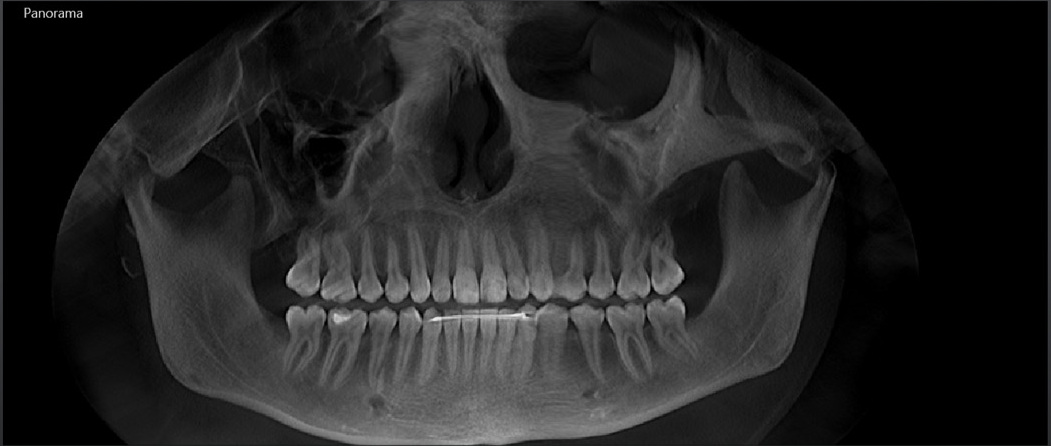
\includegraphics[width=400px]{img/anfas.jpeg}
	\caption{Снимок анфас}
	\label{fig:anfas}
\end{figure}

\begin{figure}[H]
	\centering
	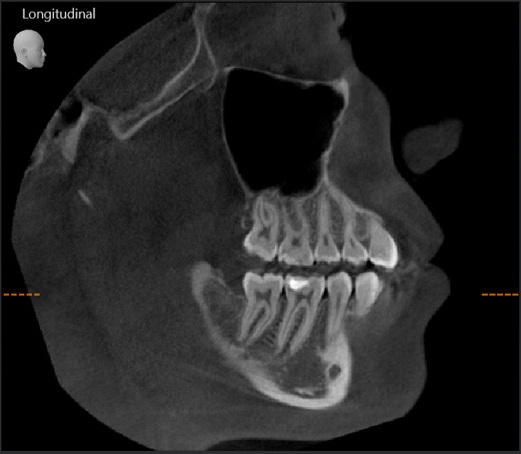
\includegraphics[width=250px]{img/profile.jpeg}
	\caption{Снимок в профиль}
	\label{fig:profile}
\end{figure}

На рисунках \ref{fig:predicted1} и \ref{fig:segmented1} соответственно приведены полученная маска и результат сегментации для снимка анфас. Как видно из снимков, никаких артефактов при проведении сегментации замечено не было.

\begin{figure}[H]
	\centering
	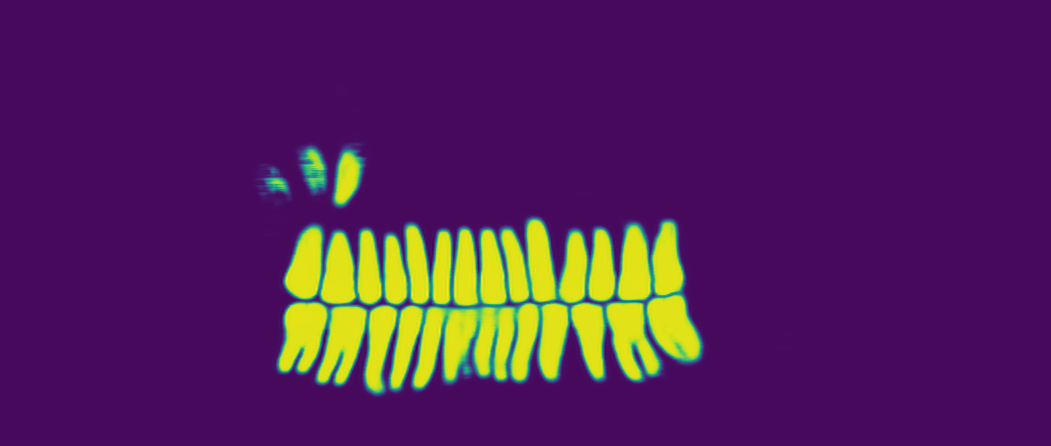
\includegraphics[width=400px]{img/predicted1.png}
	\caption{Маска для снимка анфас}
	\label{fig:predicted1}
\end{figure}

\begin{figure}[H]
	\centering
	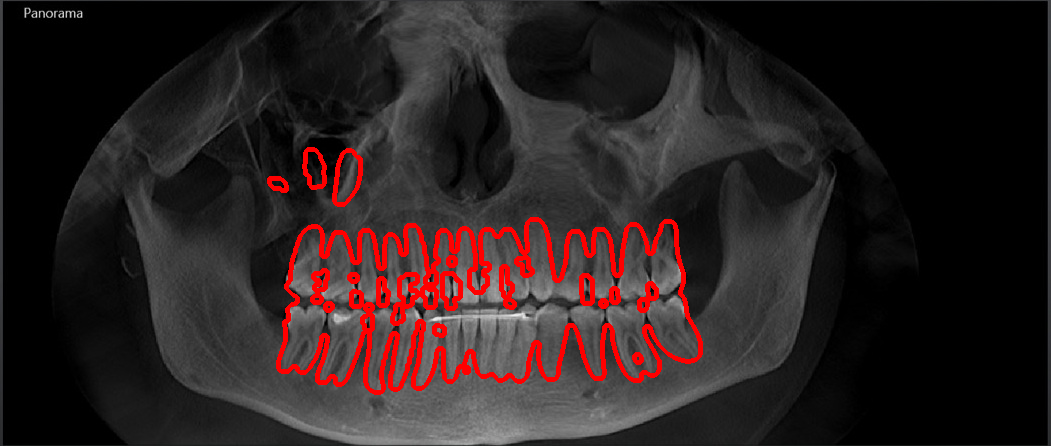
\includegraphics[width=400px]{img/segmented1.png}
	\caption{Сегментация для снимка анфас}
	\label{fig:segmented1}
\end{figure}

На рисунках \ref{fig:predicted2} и \ref{fig:segmented2} соответственно приведены полученная маска и результат сегментации для снимка в профиль. Так же как и со случаем анфас, в данном случае никаких артефактов замечено не было, маска для зубного состава была составлена корректно, за исключением небольшой области в левой верхней части снимка. Эта область является своеобразной ватермаркой снимка, такое отклонение допустимо и не затрагивает зубной состав, то есть не препятствует дальнейшему анализу полученных результатов.

\begin{figure}[H]
	\centering
	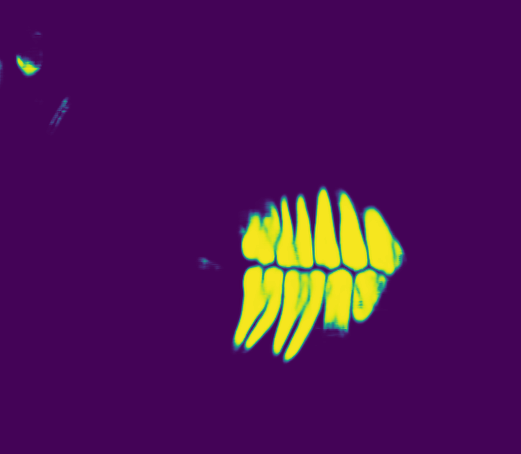
\includegraphics[width=300px]{img/predicted2.png}
	\caption{Маска для снимка в профиль}
	\label{fig:predicted2}
\end{figure}

\begin{figure}[H]
	\centering
	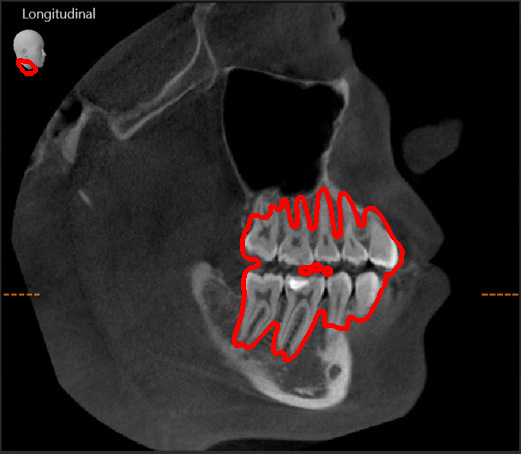
\includegraphics[width=300px]{img/segmented2.png}
	\caption{Сегментация для снимка в профиль}
	\label{fig:segmented2}
\end{figure}

\subsection{Сравнение применимости программного комплекса для снимков в разных оттенках}

В процессе обучения использовались снимки в черно--белой гамме. Помимо таких снимков, существуют аппараты, которые при снятии снимка сохраняют его в других цветовых тонах, например голубой вместо белого.

На рисунке \ref{fig:blue} представлен пример такого снимка.

\begin{figure}[H]
	\centering
	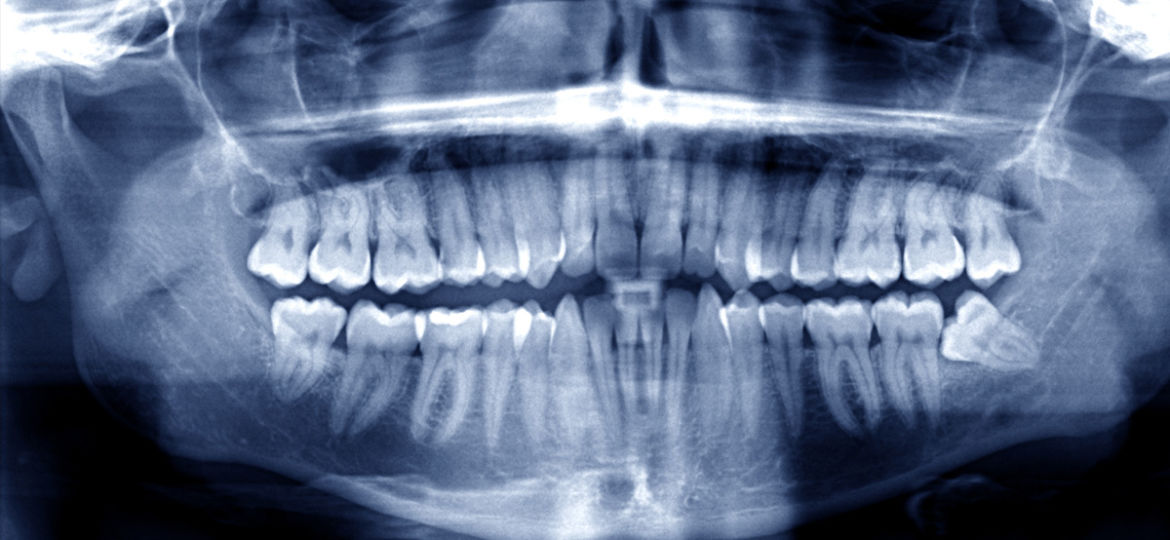
\includegraphics[width=\textwidth]{img/blue.jpeg}
	\caption{Снимок в другой цветовой гамме}
	\label{fig:blue}
\end{figure}

На рисунках \ref{fig:predicted3} и \ref{fig:segmented3} соответственно приведены полученная маска и результат сегментации для снимка в другой цветовой гамме. В целом сегментация проведена успешно, артефактов в щубном составе не наблюдается.

\begin{figure}[H]
	\centering
	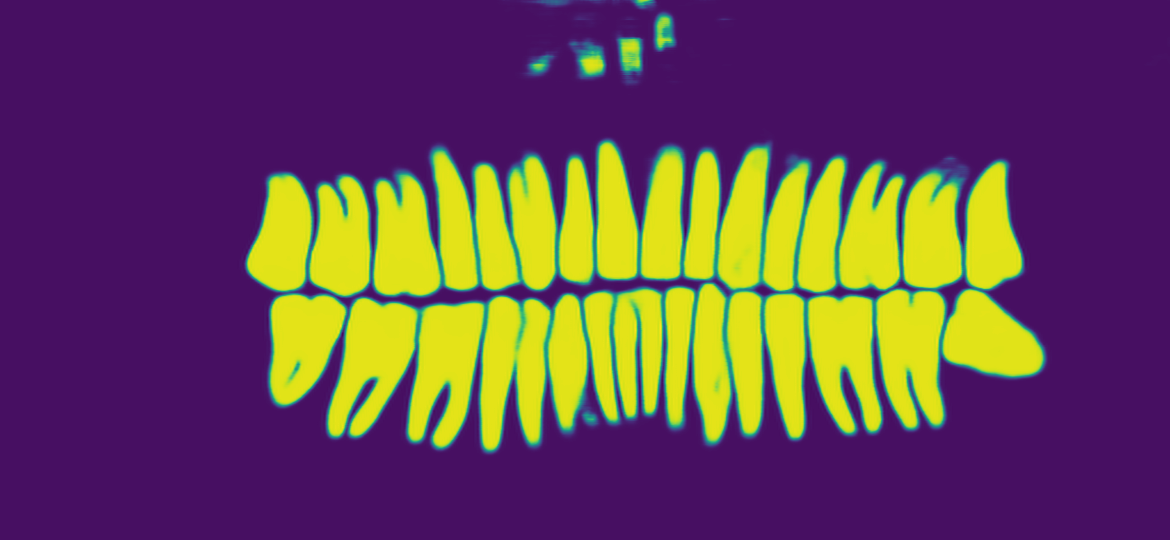
\includegraphics[width=\textwidth]{img/predicted3.png}
	\caption{Маска для снимка в другой цветовой гамме}
	\label{fig:predicted3}
\end{figure}

\begin{figure}[H]
	\centering
	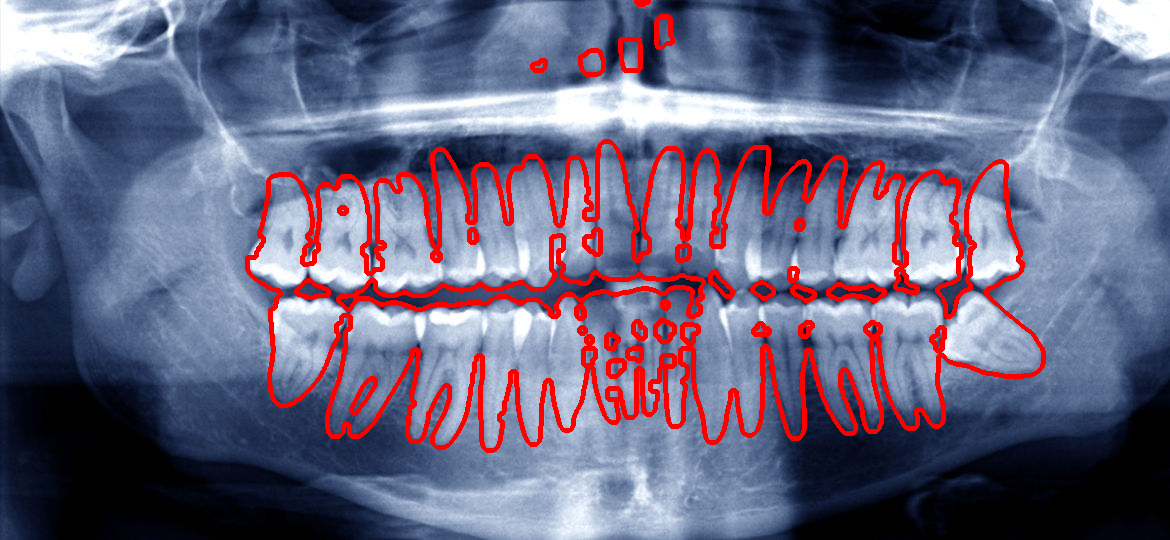
\includegraphics[width=\textwidth]{img/segmented3.png}
	\caption{Сегментация для снимка в другой цветовой гамме}
	\label{fig:segmented3}
\end{figure}

\subsection{Сравнение времени работы приложения при различном разрешении исходного снимка}

Для проведения эксперимента будем использовать снимок, представленный на рисунке \ref{fig:training}. Исходный снимок имеет разрешение $3050 \times 1250$ пикселей. Эксперимент будет проводиться на изображениях размером 100\%, 75\%, 50\% и 25\% от первоначального.

\begin{figure}[H]
	\centering
	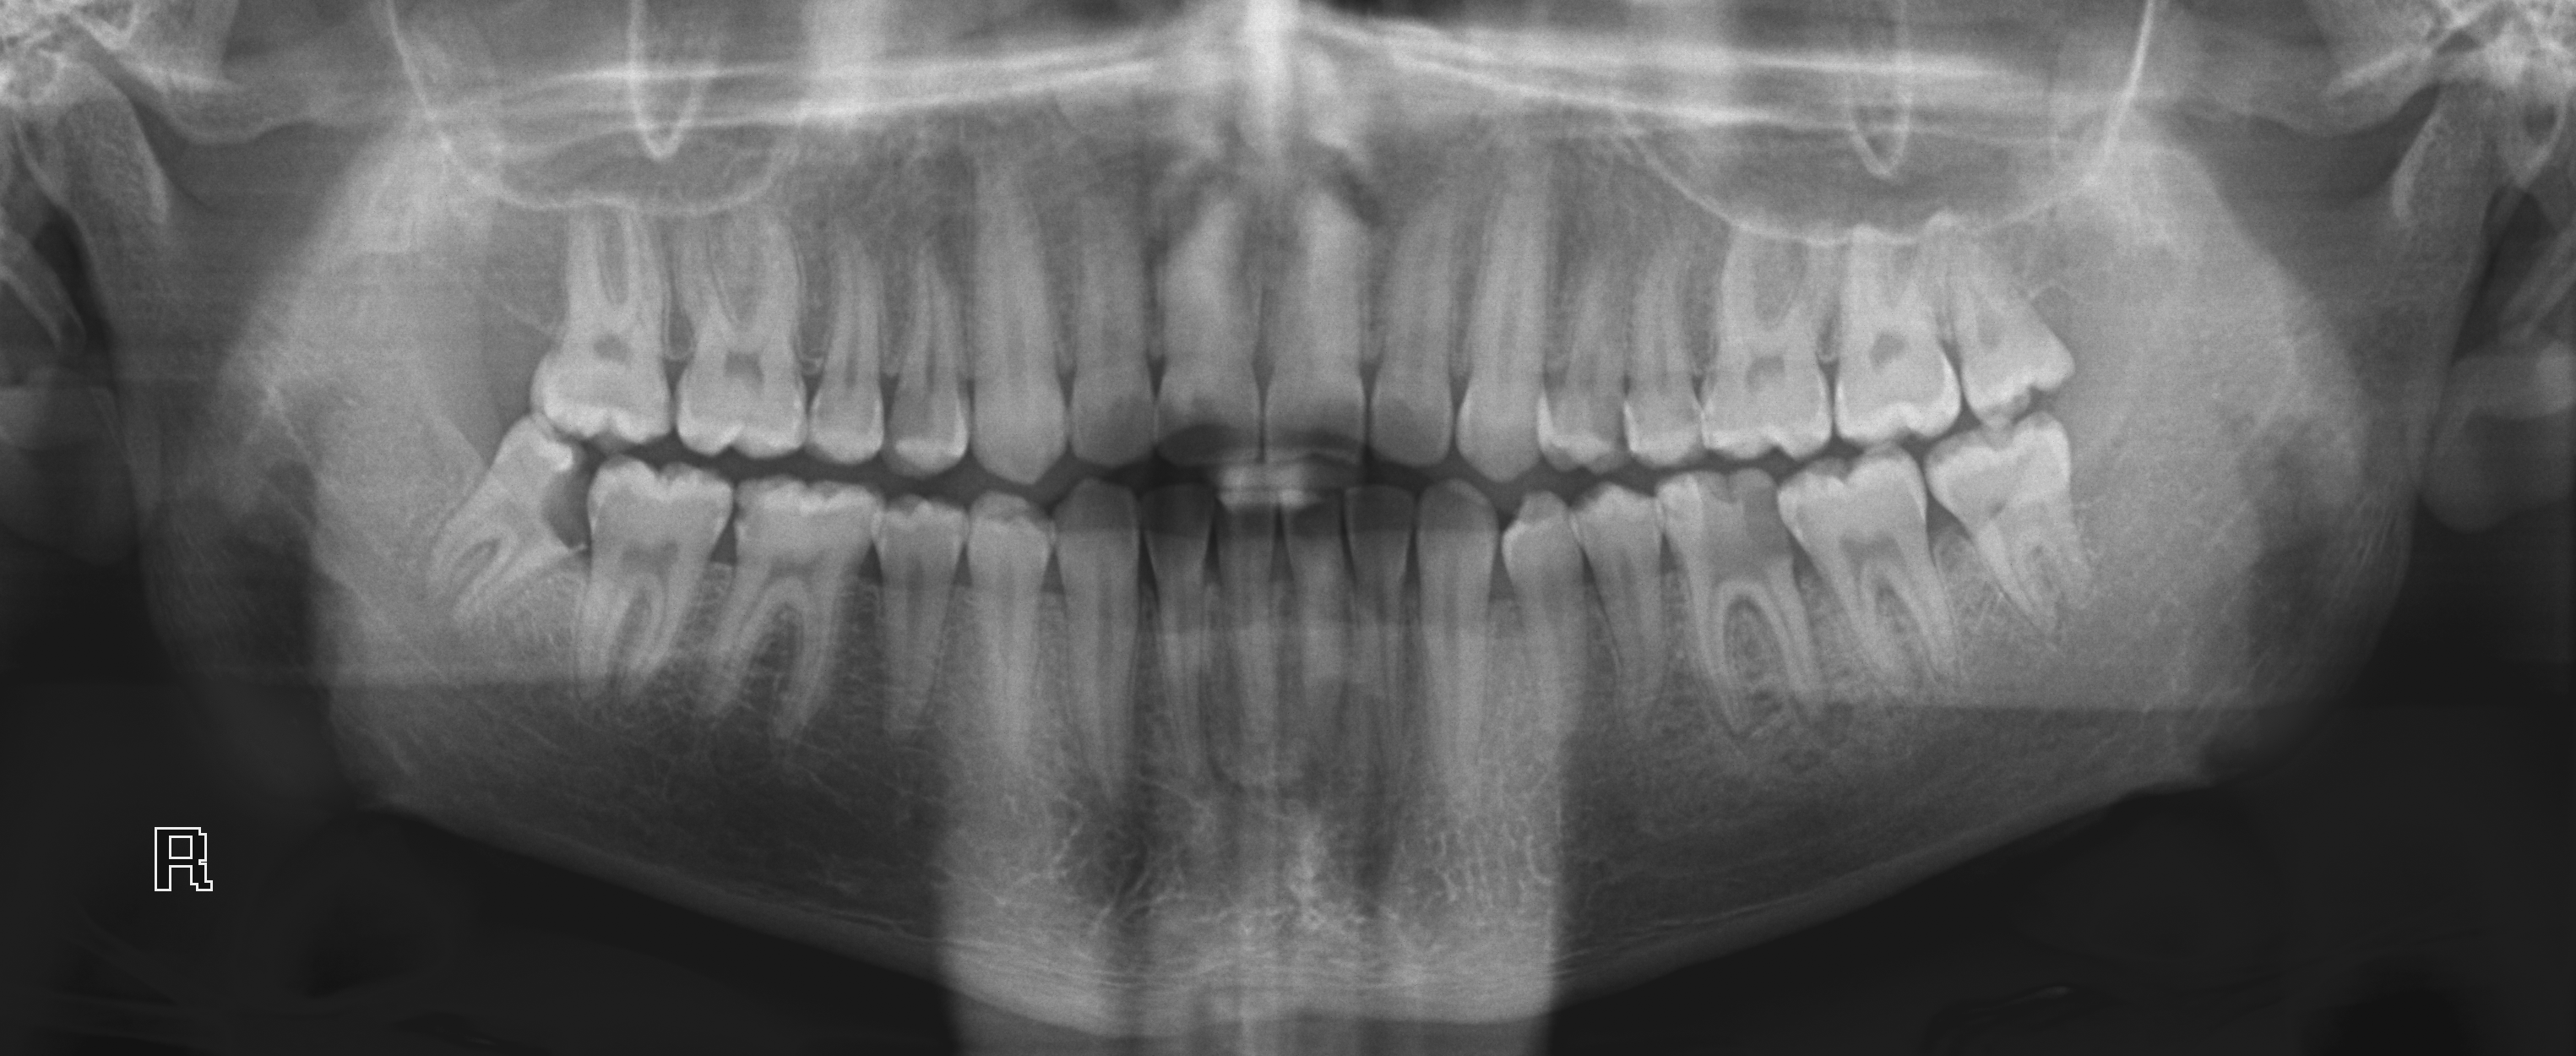
\includegraphics[width=\textwidth]{img/training.png}
	\caption{Снимок для проведения эксперимента}
	\label{fig:training}
\end{figure}

В таблице \ref{tab:run} представлена зависимость времени работы приложения от размера исходного изображения. Также эта зависимость представлена на рисунке \ref{fig:run}

% Please add the following required packages to your document preamble:
% \usepackage{graphicx}
\begin{table}[H]
	\centering
	\caption{Время работы приложения в зависимости от размера исходного изображения}
	\label{tab:run}
	\resizebox{\textwidth}{!}{%
		\begin{tabular}{|l|l|l|l|l|}
			\hline
			\textbf{Режим работы приложения} & \textbf{100\%, сек} & \textbf{75\%, сек} & \textbf{50\%, сек} & \textbf{25\%, сек} \\ \hline
			Без классификации                & 14.4                & 12.68              & 11.48              & 10.46              \\ \hline
			С классификацией                 & 17.5                & 13.18              & 11.03             & 10.37с              \\ \hline
		\end{tabular}%
	}
\end{table}

\begin{figure}[H]
	\centering
	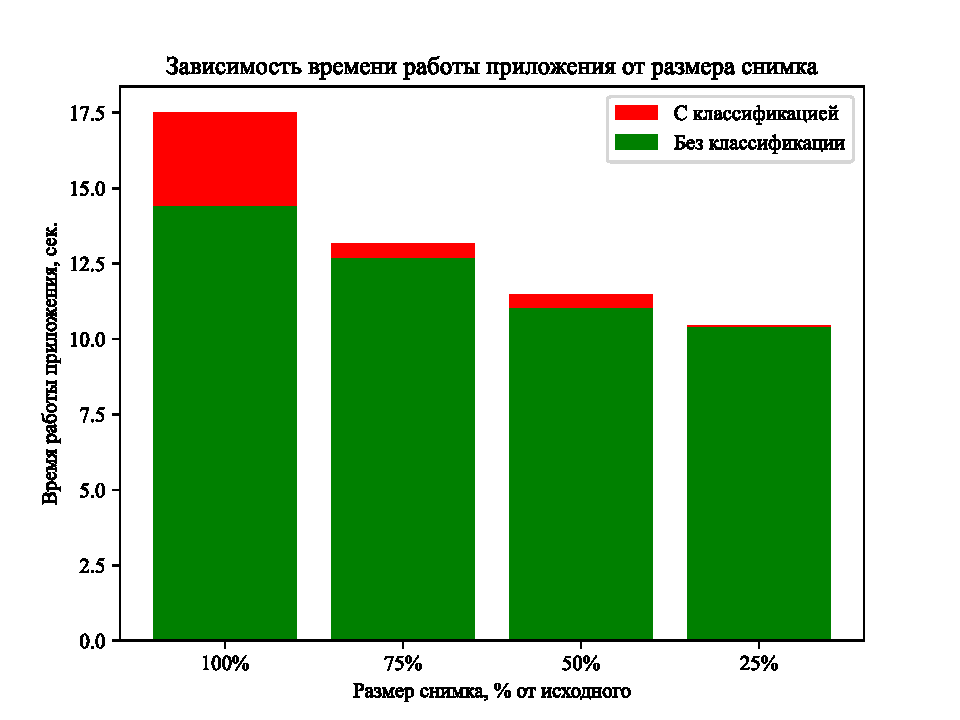
\includegraphics[width=\textwidth]{img/run.pdf}
	\caption{Зависимость времени работы приложения от размера исходного изображения}
	\label{fig:run}
\end{figure}

При уменьшении размера изображения потерь в качестве не наблюдалось, маска для сегментации всегда выделялась одинаково четко, без артефактов.

Уменьшение изображения повлияло на корректность работы классификации при помощи машины опорных векторов. Так как вектор особенностей состоял из параметров ширины и высоты зуба в пикселях, для изображений другого размера эти данные не являются корректными. Это стоит учитывать при работе с приложением.

Кроме того, классификация с уменьшением изображения занимает меньше времени. Это связано с более низкой нагрузкой на машину опорных векторов, так как приходится обрабатывать векторы, содержащие в себе меньшие числовые значения параметров модели.

\subsection{Оценка разработанного программного комплекса}

У разработанного программного комплекса можно выявить следующие достоинства и недостатки.

Достоинства:
\begin{itemize}
	\item Универсальность. Возможно использование при анализе снимков в разных проекциях, разных размеров и разных цветовых гаммах.
	\item Высокая точность. Отсутствие потери точности при сегментации при разных размерах исходного снимка.
\end{itemize}

Недостатки:
\begin{itemize}
	\item Классификация. При уменьшении разрешения снимка обнаруживаются ошибки классификации в виду неполноты данных для обучения.
\end{itemize}

\subsection*{Вывод}

Было проведено сравнение применимости разработанного программного комплекса при различных нетипичных сценариях. Протестировано быстродействие программы при использовании классификации и без ее использования. Представлены достоинства и недостатки программного комплекса.